% \vspace{-5pt}
\section{Introduction}\label{sec:ch3:intro}

 \begin{figure}[h]
\centering
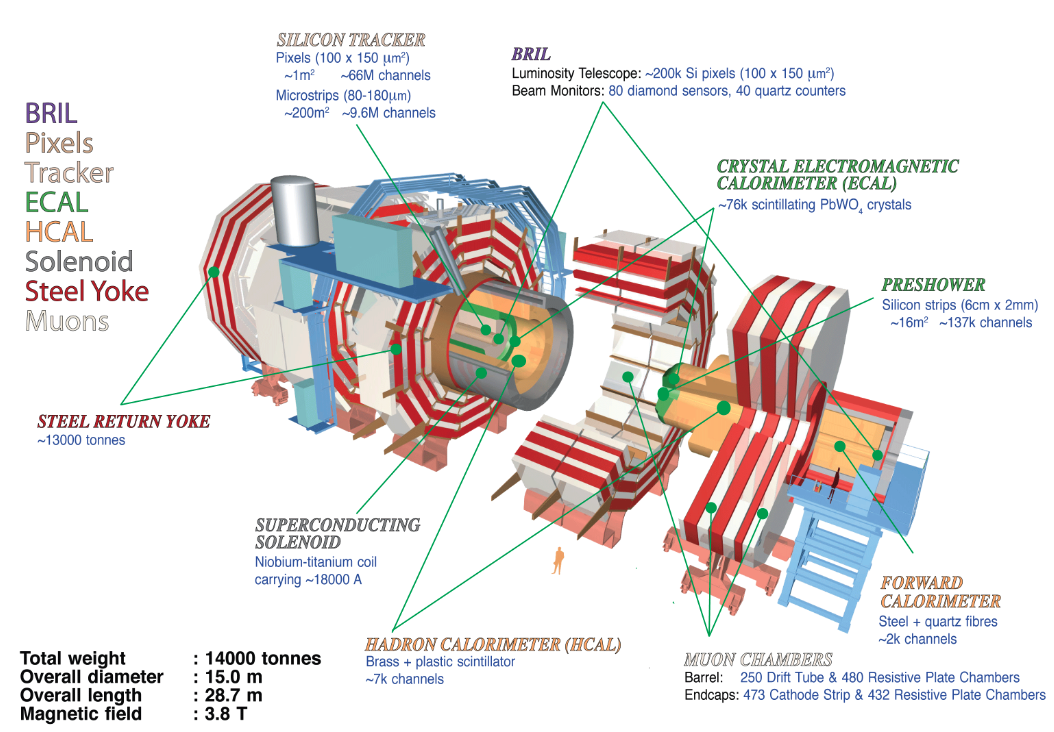
\includegraphics[width=0.8\textwidth]{figures/cms_schematic.png}
\caption{Schematic of the Compact Muon Solenoid (CMS) detector.}
\label{fig:cms}
\end{figure}

Figure \ref{fig:cms} shows the schematic of the Compact Muon Solenoid (CMS) detector. The detector is located in the Large Hadron Collider (LHC), which is depicted in the collider apparatus in Figure \ref{fig:cern}.

 \begin{figure}[h]
\centering
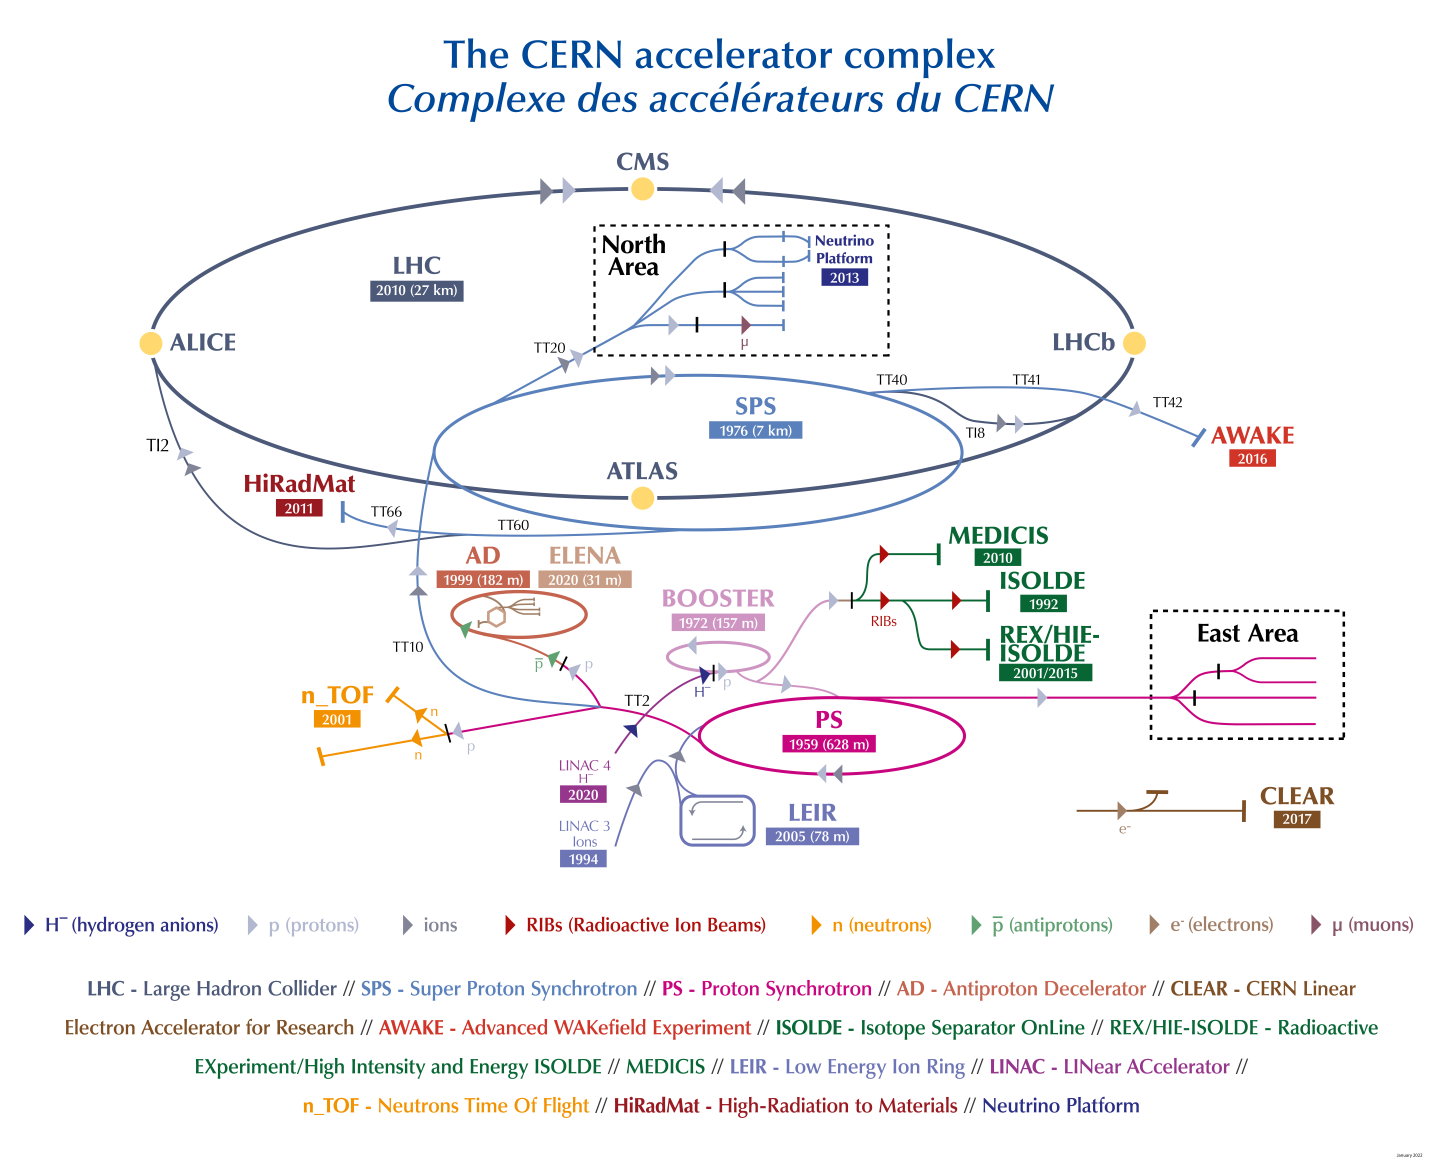
\includegraphics[width=0.8\textwidth]{figures/CCC-v2022.png}
\caption{Schematic of the collider apparatus at CERN.}
\label{fig:cern}
\end{figure}


The Large Hadron Collider (LHC) beam energy, originally at 7 TeV, now for Run 3 at 13.6 TeV, allows us to study physics at the highest energy scale in history. The collaboration also performs studies of heavy ions at 30x the energy of previous heavy ion experiments. With a luminosity for pp collisions 100x greater than previous experiments, and pp cross section of about 100 mb, measurements can be done to greater precision than ever before, and searches can probe the highest ever possible masses at the TeV scale.

The LHC contains multiple experiments. At opposite points of the collider, 27 km apart, sit ATLAS (or the experiment formerly known as A ToroidaL ApparatuS) and the Compact Muon Solenoid (CMS) experiments. The experiments perform similar searches and measurements without sharing preliminary results. This mitigates biases from experimentalists during the analyses.

The CMS detector is located at P5 at the large hadron collider~\cite{CMSExperiment}.


The CMS experiment has 5 layers. From innermost to outermost layer sits the tracker, the electromagnetic calorimeter, the hadronic calorimeter, the solenoid, and the muon chambers. These 5 layers are also referred to as "detectors", with each detector having subdetectors to make up the different geometrical portions. The CMS detector is cylindrical and so each detector has a cylindrical "barrel" region and disk-shaped "endcap" region. The Endcap regions are necessary as nearly $1/3$ of all particles cross the $1.3 < |\eta| < 3$ region.